\documentclass[12pt, a4paper]{extarticle}
\usepackage{geometry}
\geometry{
	a4paper,
	total={170mm,257mm},
	left=20mm,
	top=20mm,
	}
\usepackage{graphicx, float} % For figures
\usepackage{authblk}
\usepackage{amsmath}
\usepackage{amsmath, mathtools}
\usepackage{graphicx}
\usepackage{caption}
\usepackage{subcaption}
\usepackage{float}
\usepackage{wasysym}
\usepackage[procnames]{listings}
\usepackage{color}
\usepackage{multirow}

%title and author details
\title{Aeroelastic Analysis of Hypersonic Double-wedge Lifting Surface}
\author[1]{Koorosh Gobal}
\author[1]{(Add your name)}
\author[1]{(Add your name)}
\affil[1]{Department of Mechanical and Materials Engineering, Wright State University}
\date{} %remove date

\begin{document}

\maketitle

\abstract{}
% ===================================================================
\section{Demonstration Results}
\subsection{Linear MCK System}

\begin{equation}
	\ddot{x} + \dot{x} + x = \sin 2t
\end{equation}
\begin{figure}[H]
	\centering
	\begin{subfigure}[h]{8.0 cm}
		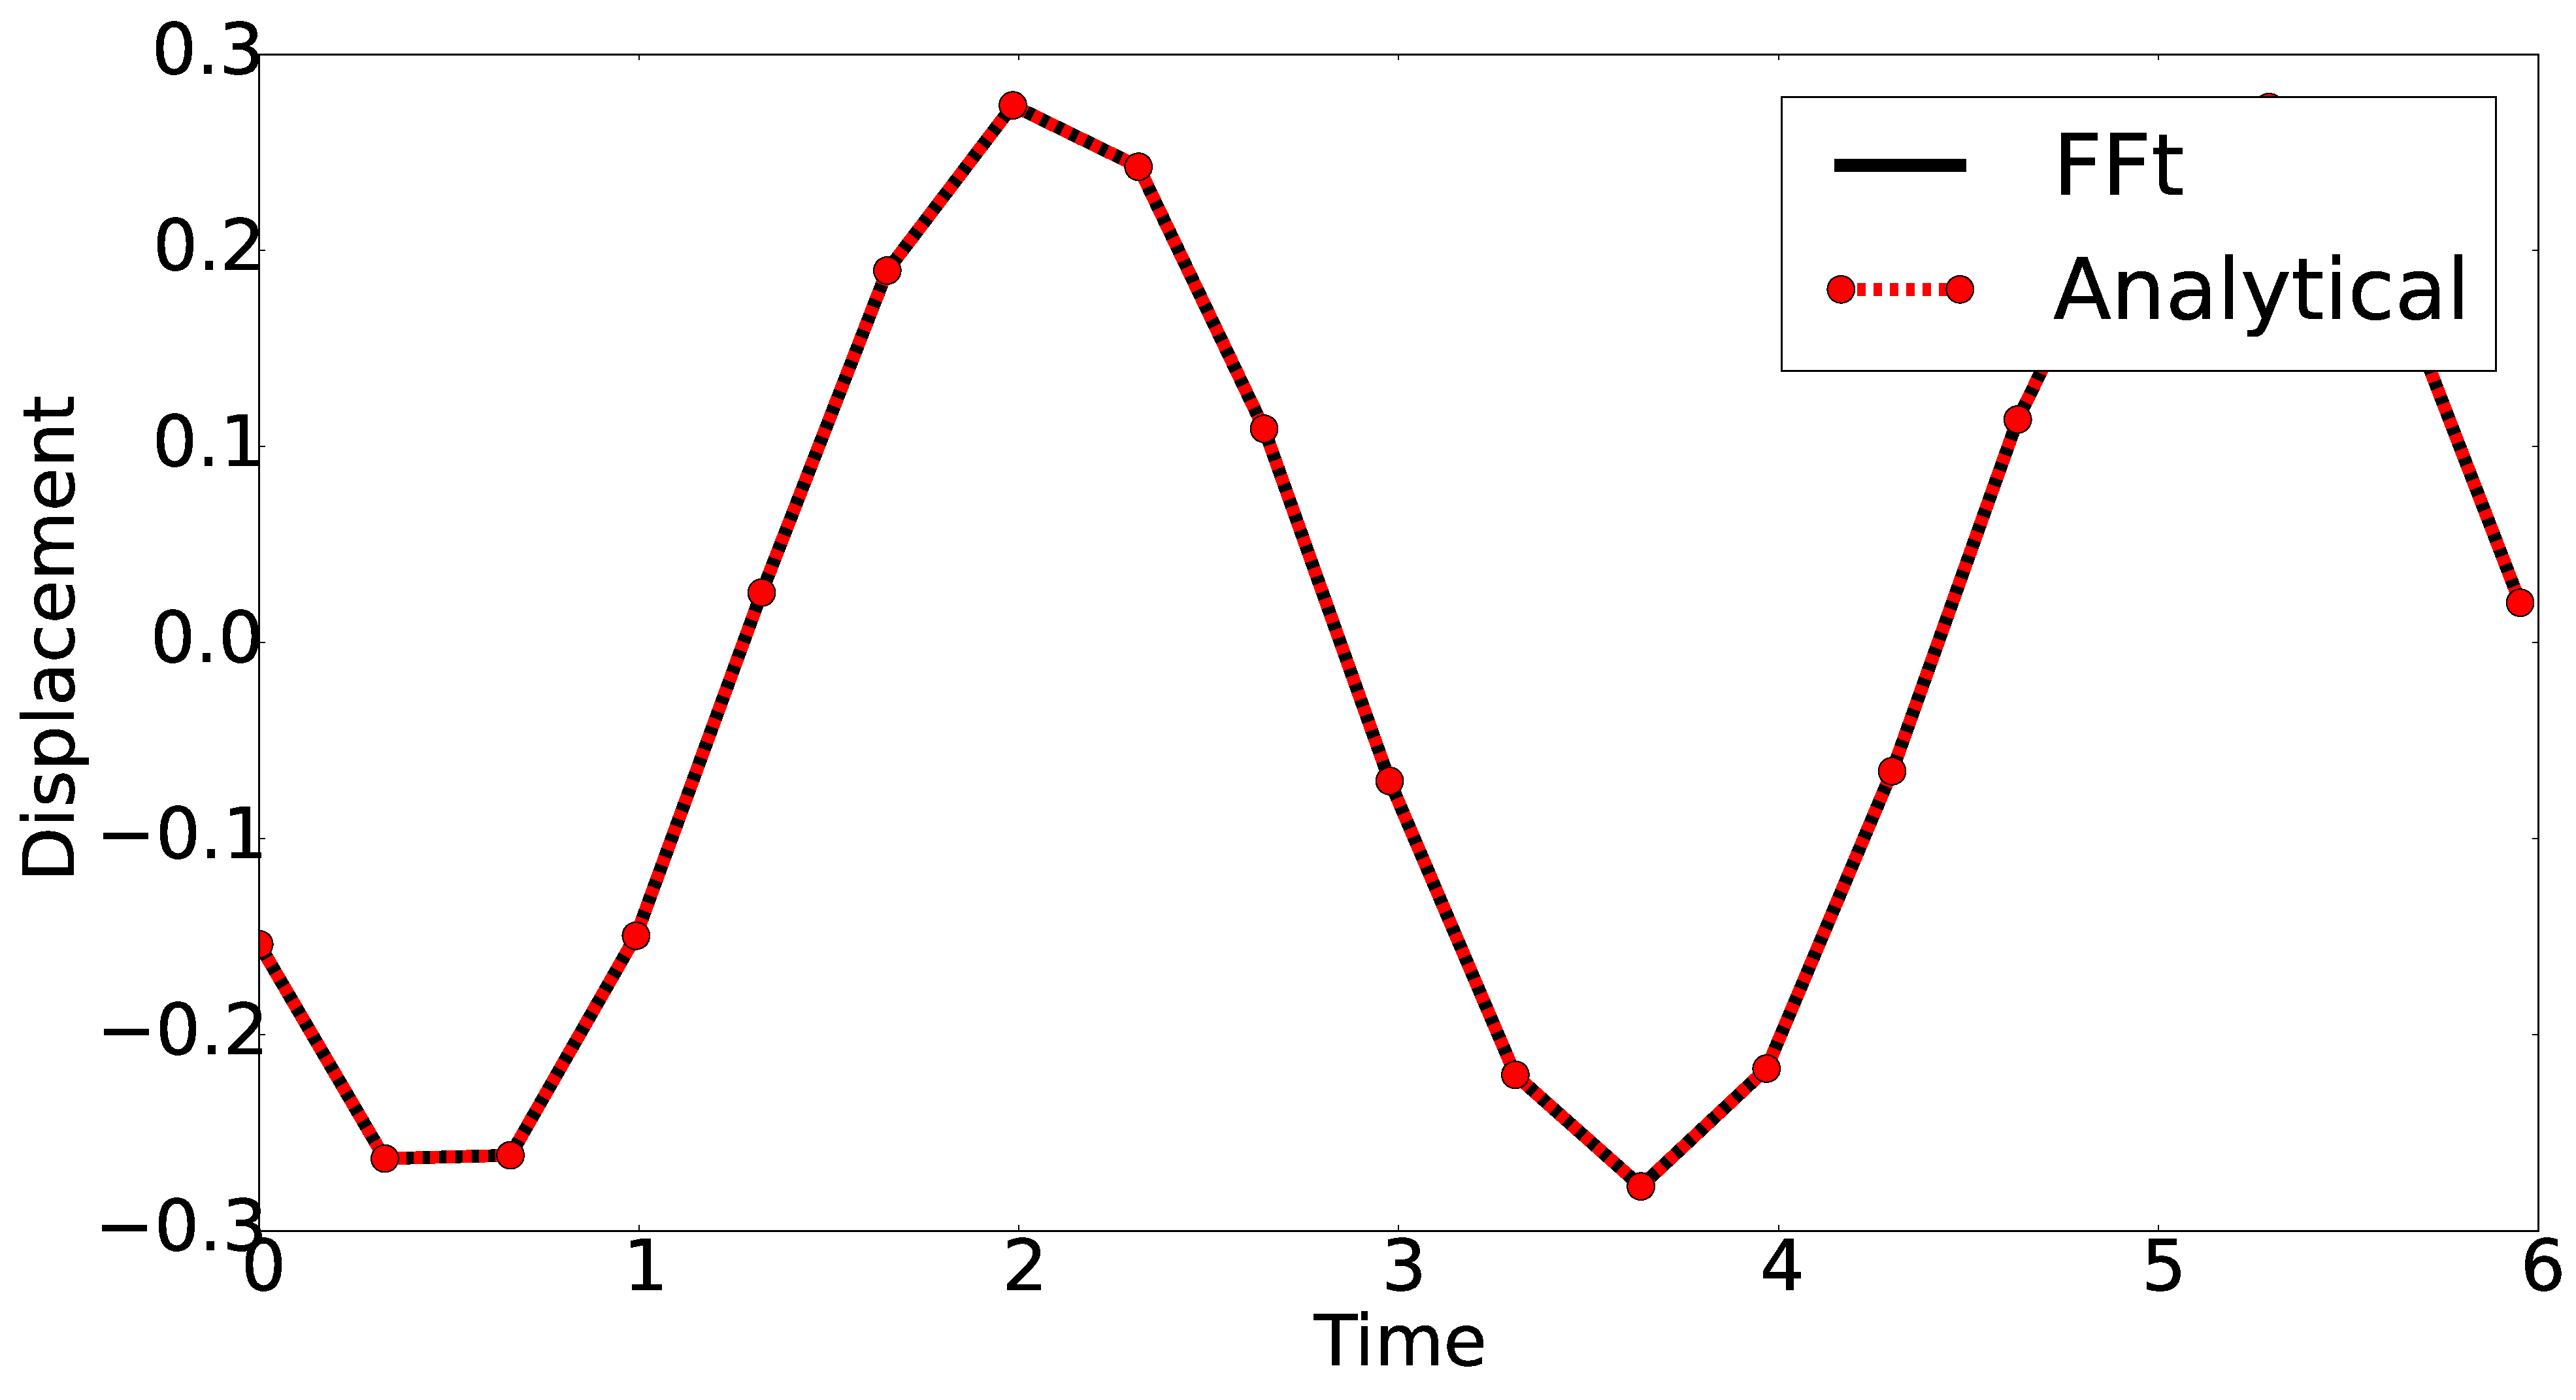
\includegraphics[width=8.0 cm]{figure/1N19.eps}
		\caption{n = 19}
	\end{subfigure}
	\begin{subfigure}[h]{8.0 cm}
        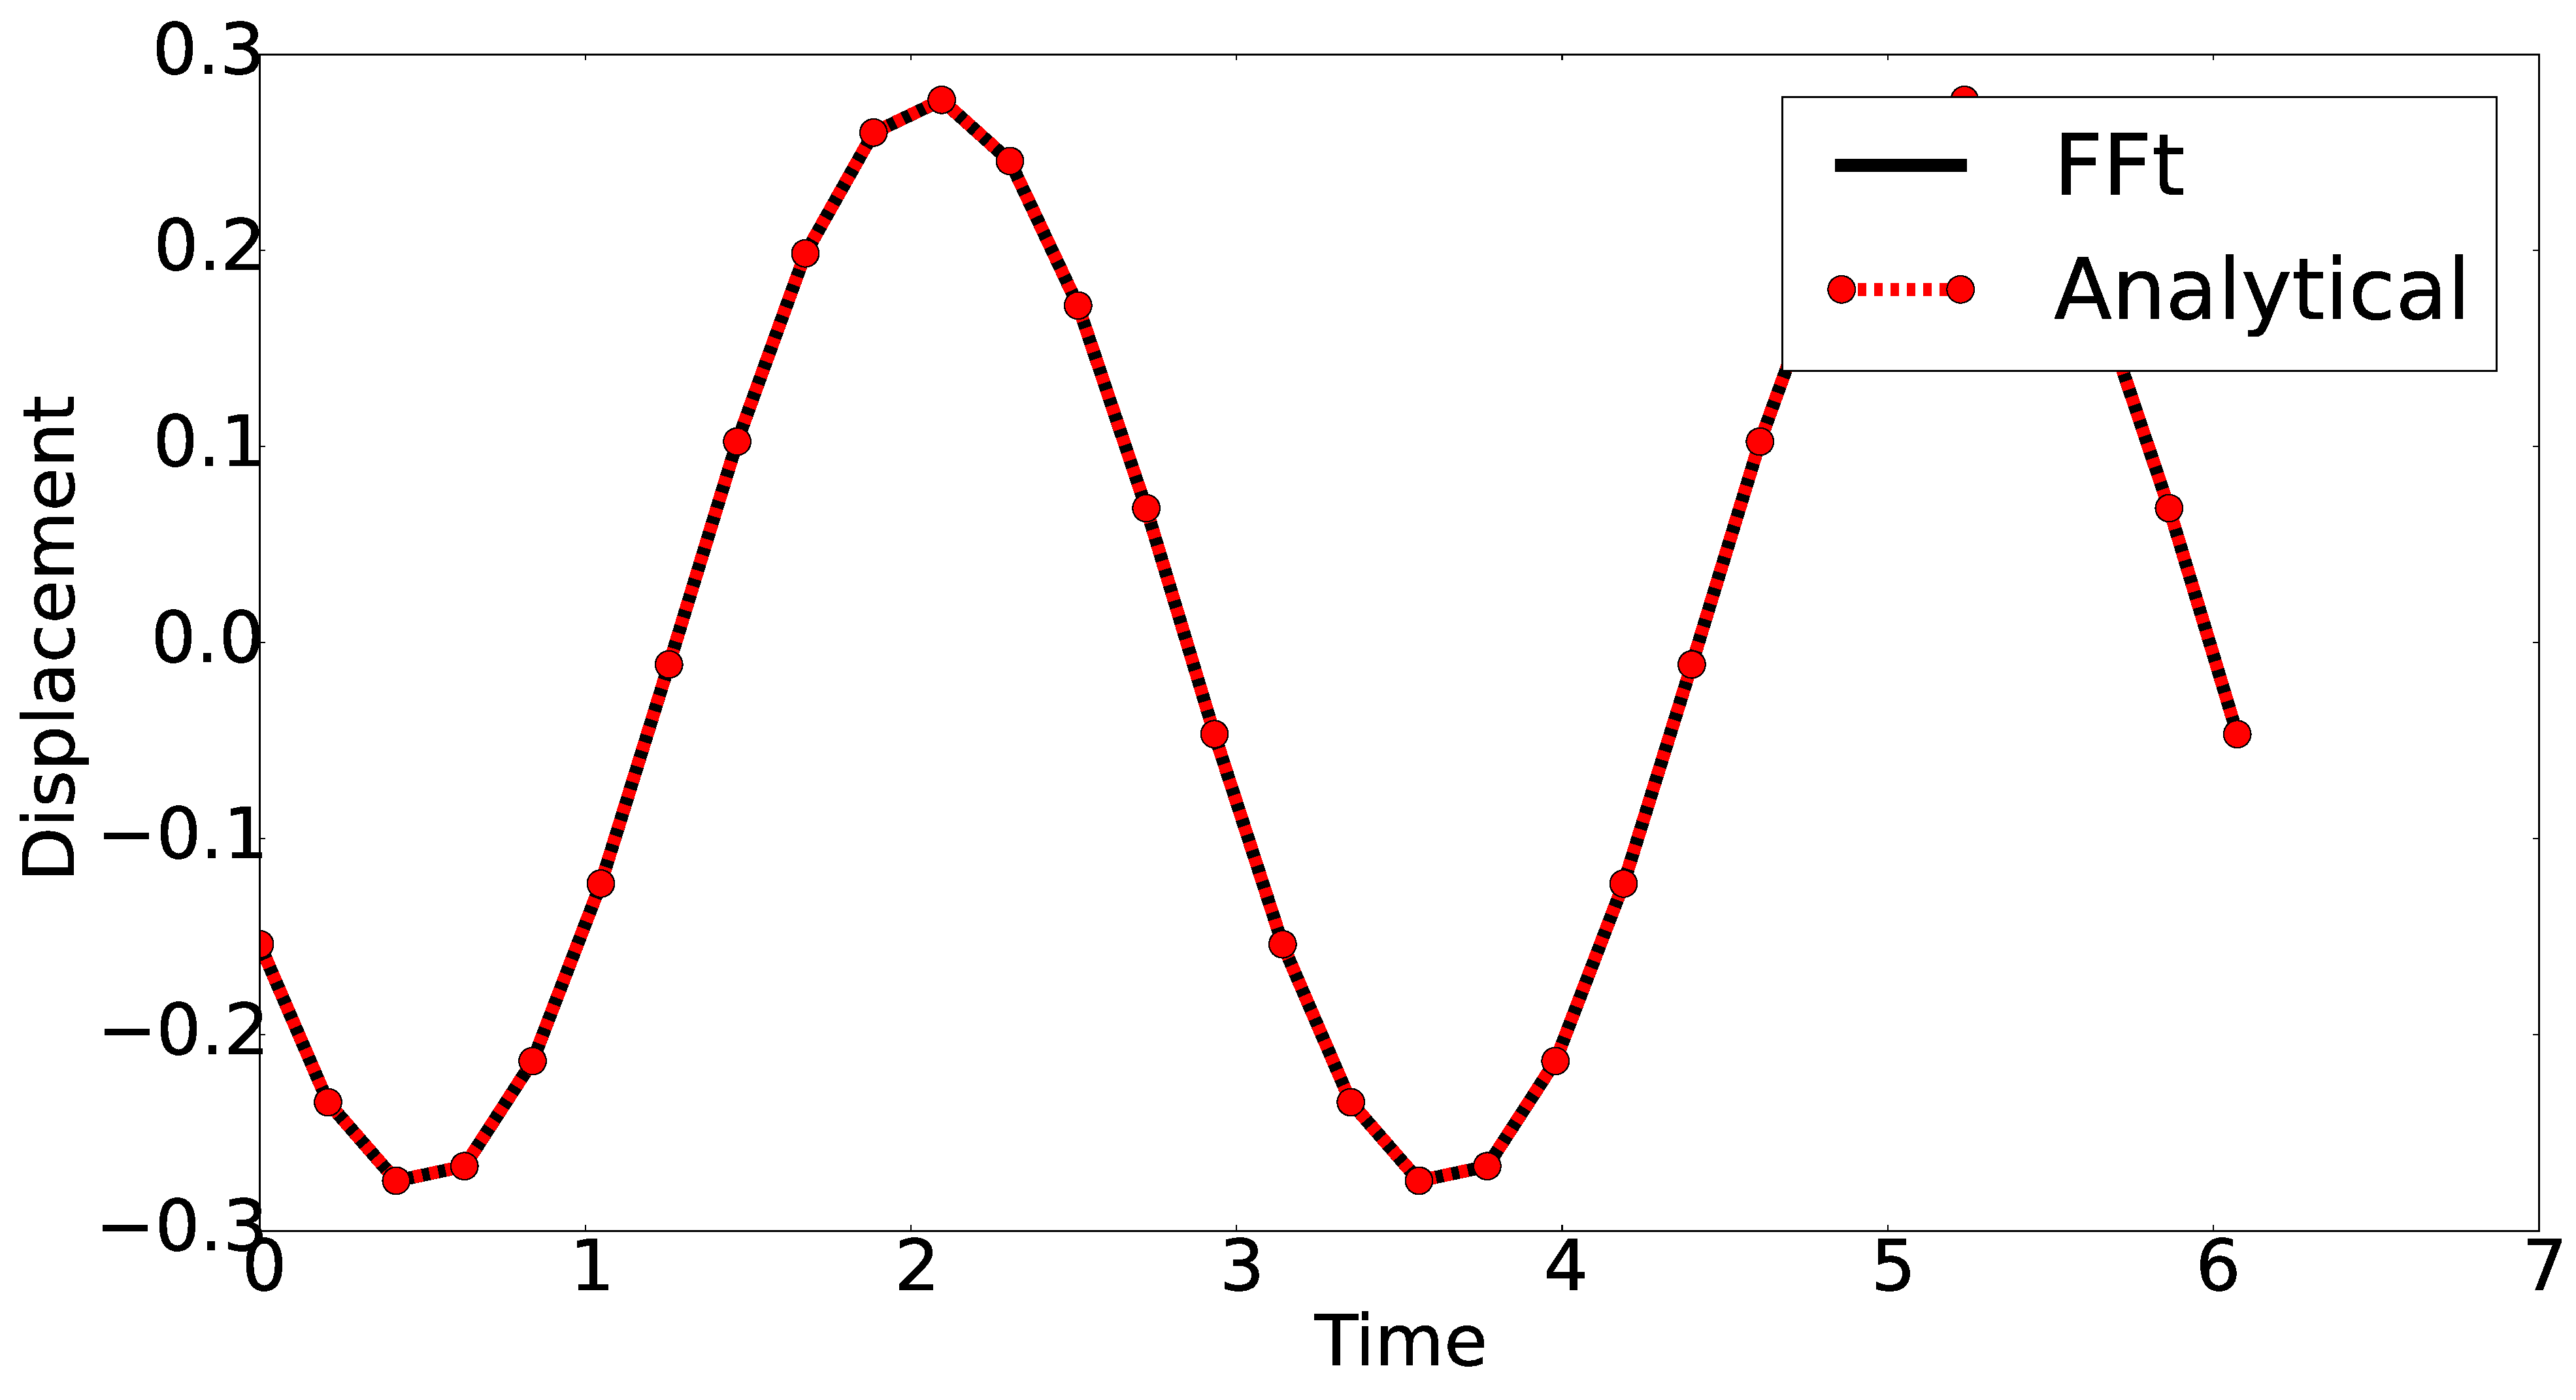
\includegraphics[width=8.0 cm]{figure/1N30.eps}
		\caption{n = 30}
    \end{subfigure}
    \caption{Comparison between HB and analytical result.}
    \label{fig:R1}
\end{figure}

\subsection{Nonlinear Oscilator}
(Problem 2.45 on page 140 of Applied Nonlinear Dynamics: Analytical, Computational, and Experimental Methods (Nayfeh))
\begin{equation}
	\ddot{x} + 2 \mu \dot{x} + \frac{g}{R} \sin x - \alpha^2 \sin x \cos x = \sin 2t
\end{equation}
mu = 0.1
g = 9.81
R = 1.0
alpha = 1
\begin{figure}[H]
	\centering
	\begin{subfigure}[h]{8.0 cm}
		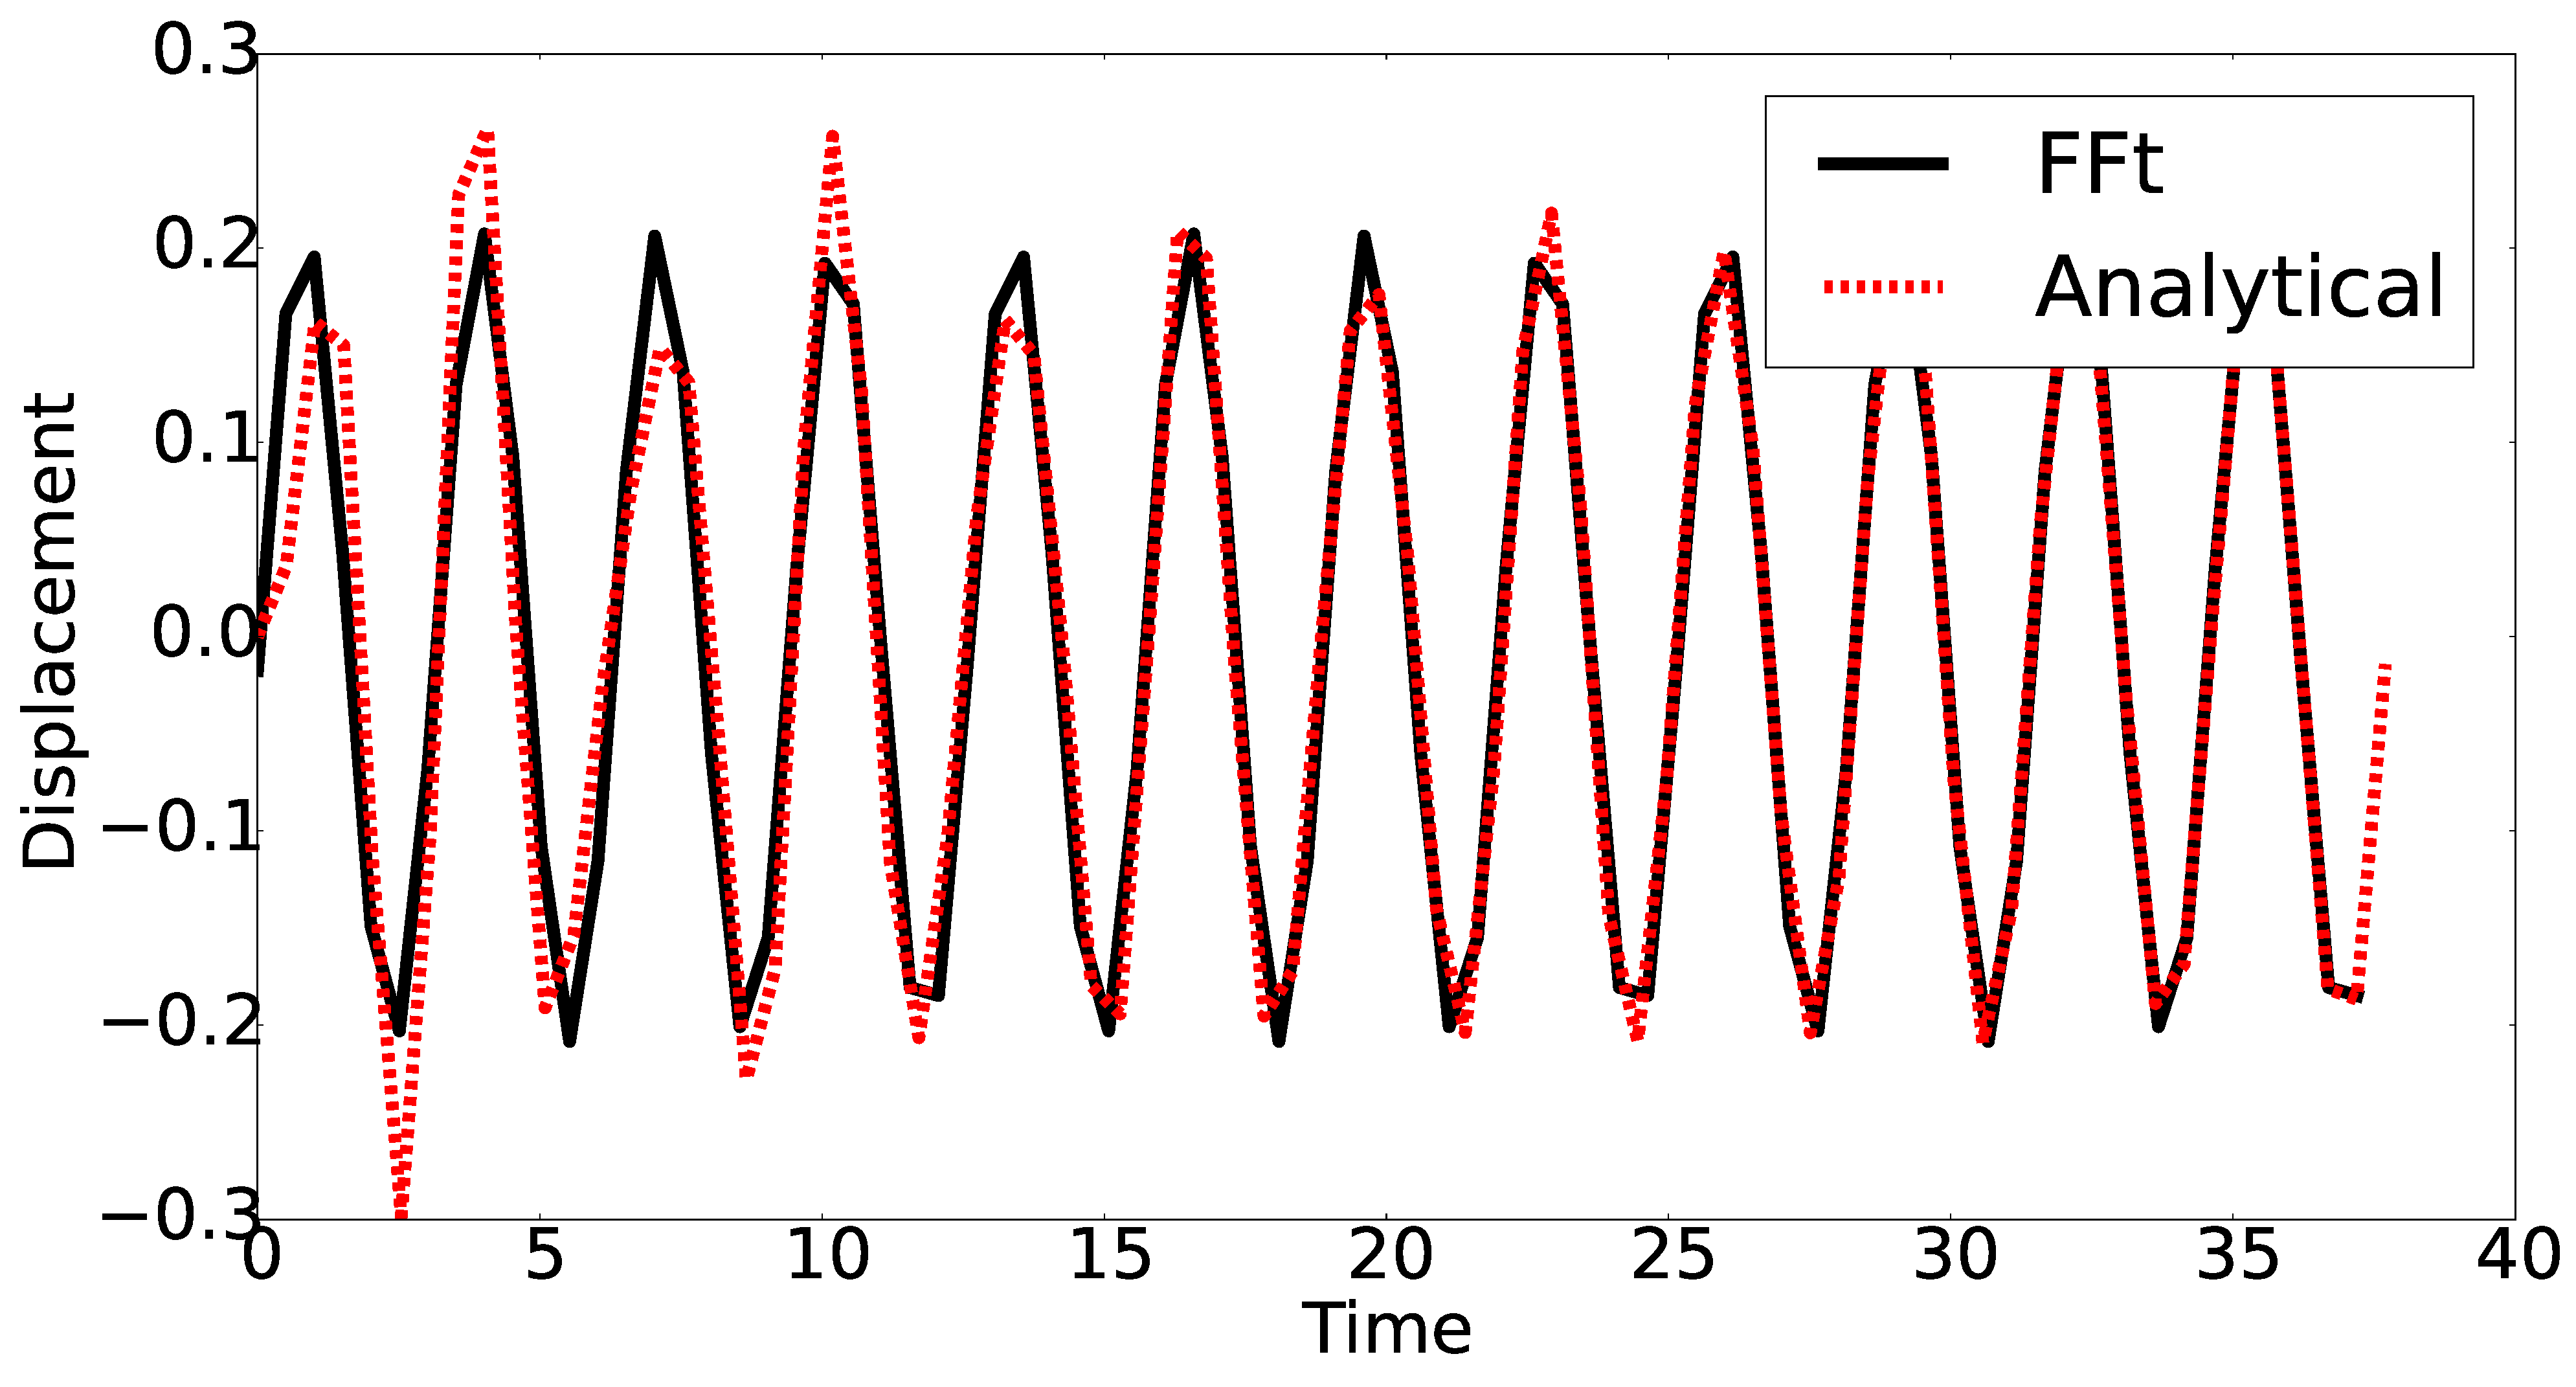
\includegraphics[width=8.0 cm]{figure/2N75.eps}
		\caption{n = 75}
	\end{subfigure}
	\begin{subfigure}[h]{8.0 cm}
        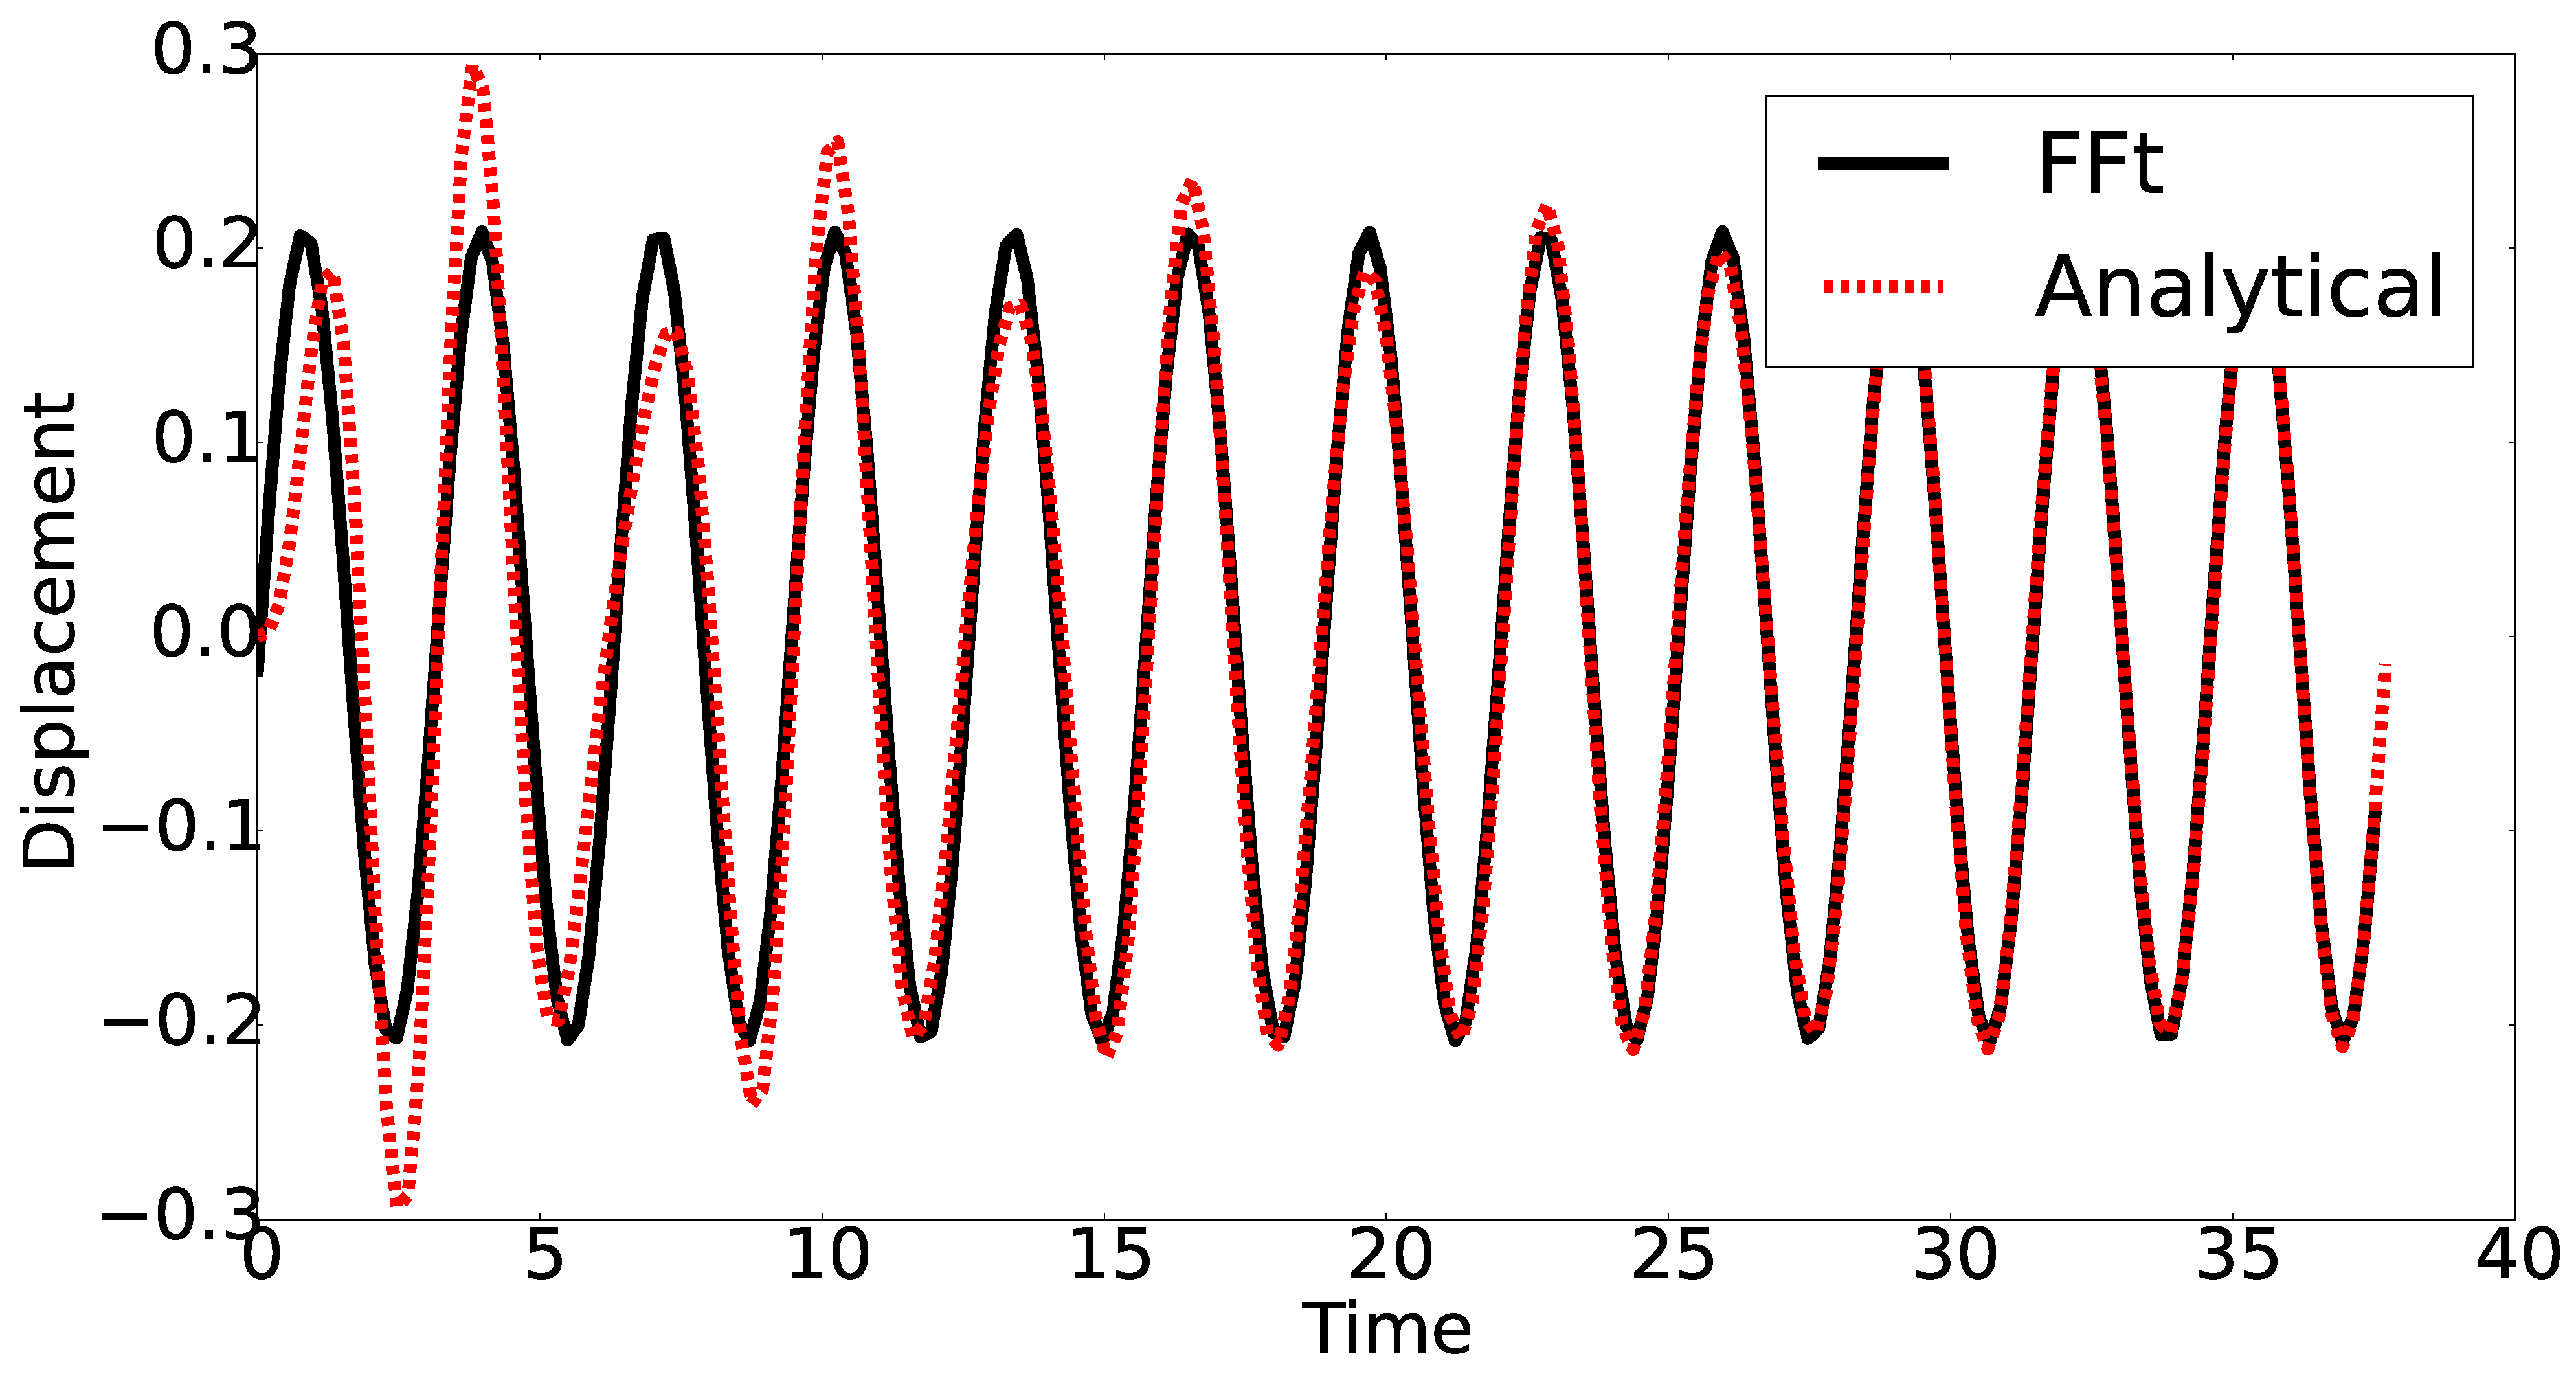
\includegraphics[width=8.0 cm]{figure/2N199.eps}
		\caption{n = 199}
    \end{subfigure}
    \caption{Comparison between HB and analytical result.}
    \label{fig:R1}
\end{figure}
\subsection{Parametrically excited Duffing Oscillator}

\begin{equation}
	\ddot{x} + x + \epsilon \left[ 2 \mu \dot{x} + \alpha x^3 + 2 k x \cos \omega t \right] = \sin 2t	
\end{equation}
epsilon = 1.0
mu = 1.0
alpha = 1.0
k = 1.0
omega = 2.0
\begin{figure}[H]
	\centering
	\begin{subfigure}[h]{8.0 cm}
		
\includegraphics[width=8.0 cm]{figure/3N20.eps}
		\caption{n = 20}
	\end{subfigure}
	\begin{subfigure}[h]{8.0 cm}
        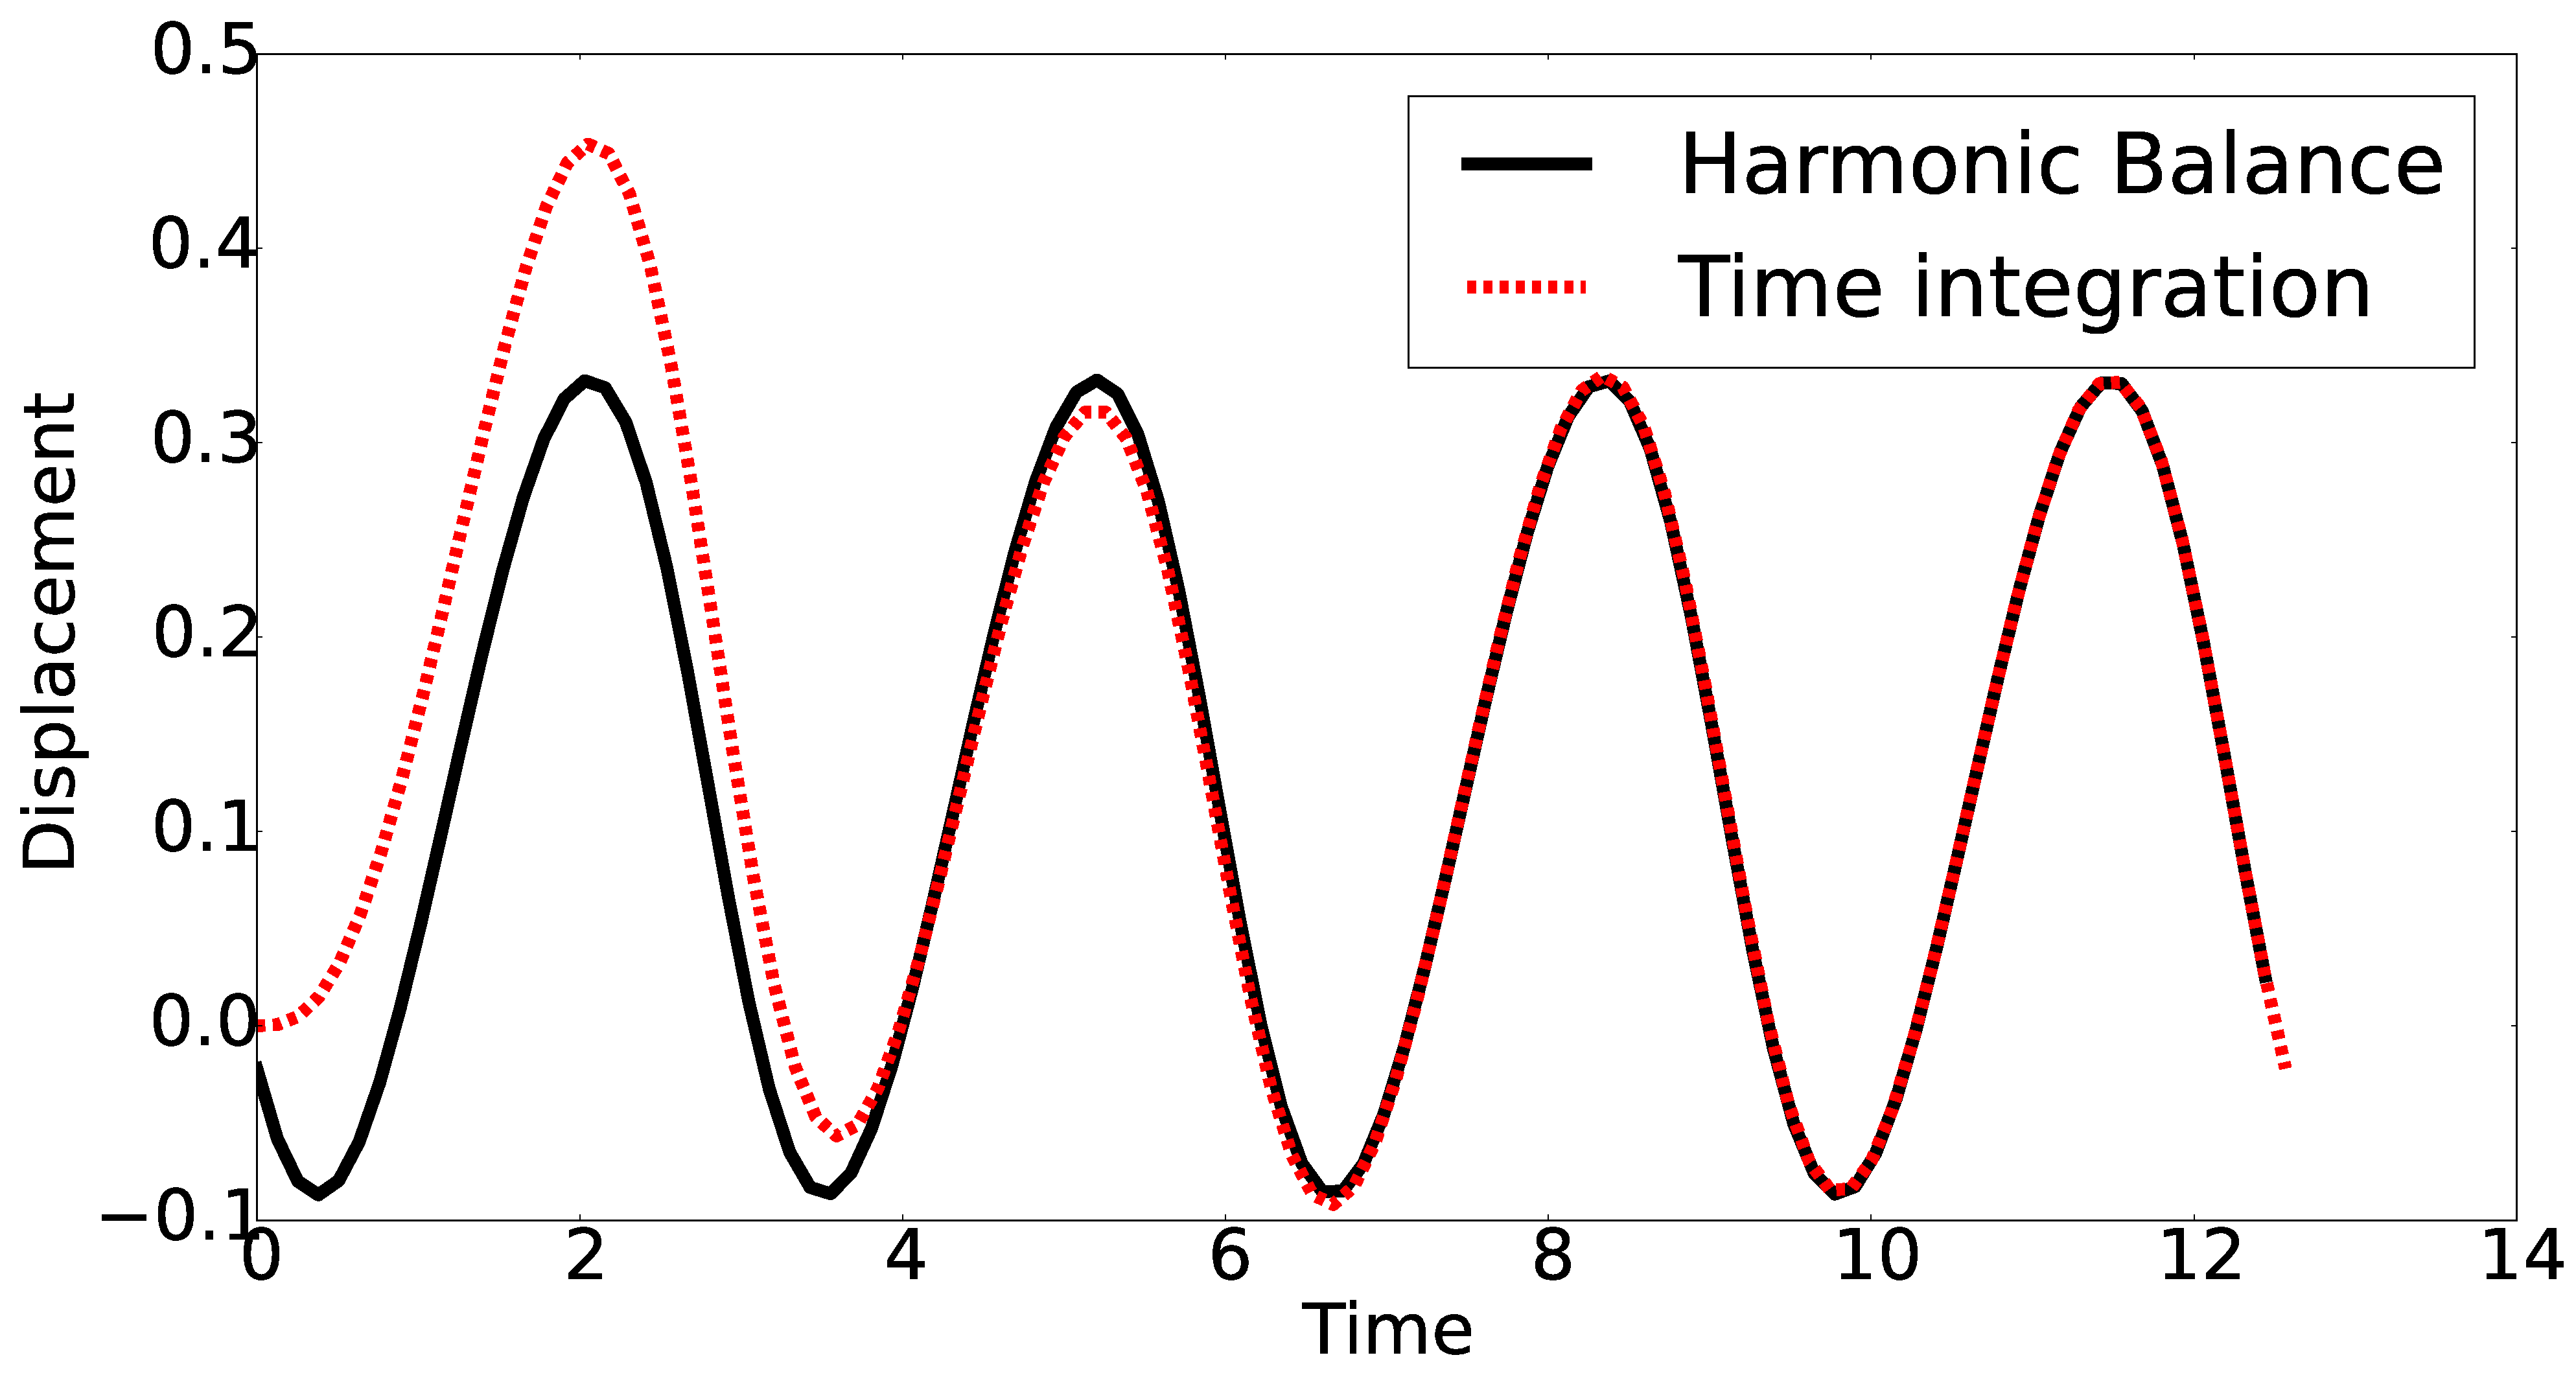
\includegraphics[width=8.0 cm]{figure/3N99.eps}
		\caption{n = 99}
    \end{subfigure}
    \caption{Comparison between HB and analytical result.}
    \label{fig:R1}
\end{figure}
\subsection{Hypersonic Flutter}
The governing equation can be written as

\begin{equation}\label{eq:GE}
	m\ddot{\theta} + k \theta = f(\theta, t)
\end{equation}

where $m$ is the mass of airfoil, $k$ is the stiffness, $\theta$ is the angle of attack and $f$ is the aerodynamic load. We use the Piston Theory to calculate the aerodynamic load acting on the airfoil. The pressure distribution on the airfoil can be written as follows

\begin{equation}\label{eq:pistonTheory}
	\frac{P(x, t)}{P_\infty} = \left( 1+ \frac{\gamma - 1}{2} \frac{v_n}{a_\infty} \right)^{\frac{2 \gamma}{\gamma - 1}}
\end{equation}

where $P(x, t)$ is the pressure at point $x$ on the airfoil, $P_\infty$ is the free stream pressure, $\gamma$ is the ratio of specific heats and $a_\infty$ is the speed of sound. $v_n$ is calculated using the following equation.

\begin{equation}\label{eq:definitionOfVn}
	v_n = \frac{\partial Z(x,t)}{\partial t} + V \frac{\partial Z(x,t)}{\partial x}
\end{equation}

where $V$ is the free stream velocity and $Z(x,t)$ is the position of airfoil surface. The position of airfoil surface can be related to the angle of attack using the following equation:

\begin{equation}\label{eq:definitionOfZ}
	Z(x,t) = M_r\left( \theta(t) \right) Z_0(x)
\end{equation}

where $M_r$ is the rotation matrix, and $Z_0(x)$ is the initial shape of the airfoil.  As can be seen here, the location of surface at time $t$ only depends on the angle of attach at that time, $\theta(t)$. The rotation matrix is defined as

\begin{equation*}
	M_r = 
	\begin{bmatrix}
		\cos \theta & -\sin \theta \\
		\sin \theta & \cos \theta
	\end{bmatrix}
\end{equation*}

By expanding Equation \eqref{eq:pistonTheory}, and substituting for $Z(x,t)$ from Equation \eqref{eq:definitionOfZ}, Equation \eqref{eq:GE} can be rewritten as

\begin{subequations}
\begin{gather}
	m\ddot{\theta} + k \theta = 
	\oint_{airfoil} P_\infty
	\left[
	\gamma \frac{v_n}{a_\infty} +
	\frac{\gamma (\gamma + 1)}{4} \left( \frac{v_n}{a_\infty}\right)^2 +
	1
	\right] ds
	\\
	v_n = 
	\frac{\partial M_r(\theta)}{\partial t}Z_0(x) + V M_r(\theta)\frac{\partial Z_0(x)}{\partial x}
\end{gather}\label{eq:GEfull}
\end{subequations}

Equation \eqref{eq:GEfull} needs to be solved for $\theta$ using Harmonic Balance method.
% ===================================================================
\bibliographystyle{unsrt}
\bibliography{ref}
\end{document}